\section{Physical data structures
and query optimization}
\url{../other/professor's slides/3_PhysicalDatabases.pdf}
\begin{center}
    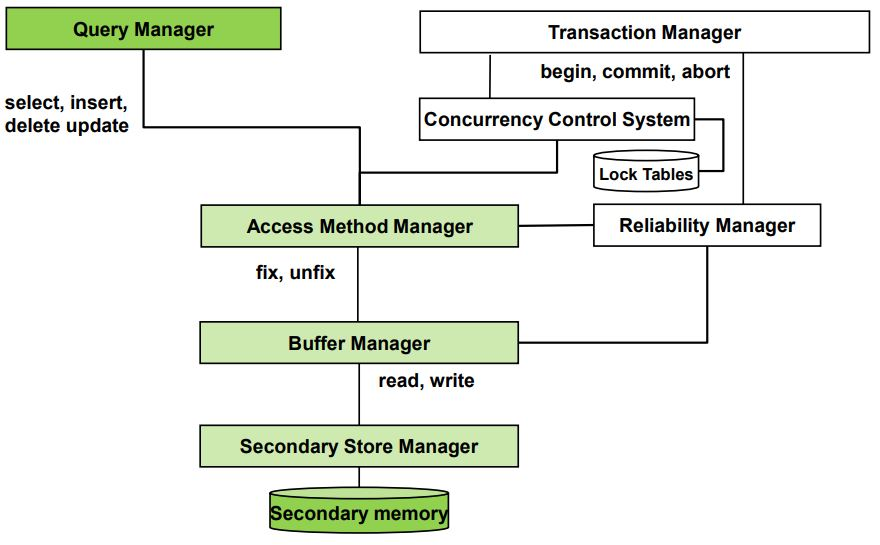
\includegraphics[height=6cm]{../arguments/Querymanagement.JPG}
\end{center}
\subsection{Data Access and Cost Model}
\subsubsection{Main and secondry memory}
Data bases have two memories: \textbf{main memory} and \textbf{secondary memory}.\newline
\newline
Databases must be stored mainly in files onto secondary memory for two reasons: size and persistance.\newline
\newline
Data stored in secondary memory can only be used if first transferred to the main memory.\newline
\newline
Second memory devices are organized in \textbf{blocks} of \textbf{fixed} length. Main memory is instead organized in \textbf{buffer}, that is a large area of memory organized in \textbf{pages}. We assume that the size of a page is the size of a block\newline
\newline
The cost of an access to secondary memory is usually considered 4 orders of magnitude higher than that to main memory.
\subsubsection{DBMS and file system}
\textbf{File System (FS)}: component of the OS which manages access to secondary memory.\newline
\newline
DBMSs make limited use of FS functionalities: the DBMS directly manages the file organization, both in terms of the distribution of records within blocks and with respect to the internal structure of each block. A DBMS may also control the physical allocation of blocks onto the disk for faster sequential reads.
\subsection{Physical access structures}
\textbf{Access methods}: software modules that provide data access and manipulation (store and retrieve) \textbf{primitives} for each physical access structure.\newline
\newline
Access methods have their own data structures to organize data:
\begin{itemize}
    \item each table is stored into \textbf{exactly one primary} physical access structure;
    \item each table may have \textbf{one or more optional secondary} access structure.
\end{itemize}
\ \newline
\textbf{Primary structure}: it contains all the tuples of a table. The main purpose is to actually store the table content.\newline
\newline
\textbf{Secondary structures}: are used to index primary structure, and only contain the values of some fields, interleaved with pointers to the blocks of the primary structure. The main purpose is to speed up the search for specific tuples, according to some search criterion.\newline
\newline
[off topic: An example of primary and secodnary structure may be an array (primary structure) contianing the data and a red and black tree of pointers (secondary structure) pointing to the array's cells.]\newline
\newline
Three main \textbf{types of data access structures}:
\begin{itemize}
    \item \textbf{Sequential} structures;
    \item \textbf{Hash-based} structures;
    \item \textbf{Tree-based} structures.
\end{itemize}
\subsubsection{Blocks and tuples}
\textbf{Block}: the "physical" components of files. The size of a block is typically fixed and depends on the file system and on how the disk is formatted.\newline
\newline
\textbf{Tuples}: the "logical" components of tables. The size of a tuple (also called record) depends on the database design and is typically variable within a file.
\newline
\newline
\textbf{Organization of tuples within blocks/pages}:
\begin{center}
    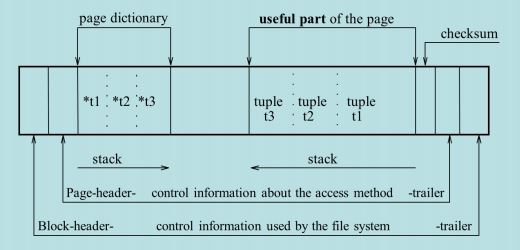
\includegraphics[height=4cm]{../arguments/organizationoftuples.JPG}
\end{center}
\begin{itemize}
    \item Block header and trailer with control information used by the file system;
    \item Page header and trailer with control information about the access method;
    \item A page dictionary, which contains pointers (offset table) to each elementary item of useful data contained in the page;
    \item A useful part, which contains the data;
    \item A checksum, to detect corrupted data.
\end{itemize}
\textbf{Block factor (B)}: the number of tuples within a block
\[
    B = floor\left(\frac{\text{size of blok}}{\text{avarage size of a tuple}}\right)
\]
\subsubsection{Page manager primitives}
\begin{itemize}
    \item \textbf{Insertion and update of a tuple}: may require a reorganization of the page or usage of a new page;
    \item \textbf{deletion of a tuple}: often carried out by marking the tuple as "invalid";
    \item \textbf{access to a field of a particular tuple}: identified according to an offset w.r.t. the beginning of the tuple and the lenght of the field itself.
\end{itemize}
\subsubsection{Sequential access structures}
Sequential structures is a sequential arrangement of tuples in the secondary memory.\newline
\newline
Three cases:
\begin{itemize}
    \item \textbf{Entry-sequenced} organization: sequence of tuples dictated by their order of entry. Optimal for space occupancy and carrying out sequntial reading and writing, non optimal with respect to searching specific data units.
    \item \textbf{Array} organization: the tuples are arranged as in array, they can be accessed through an index. Possible only when tuples are of fixed lenght.
    \item \textbf{Sequentially-ordered} organization: tuples ordered according to the value of a key (one or more attributes). The main problem are related to insertion of new tuples and updates, reordering techniwques are needed for the tuples already present.
\end{itemize}
\subsubsection{Hash-based access structures}
the hash-based access structures are an efficient \textbf{associative access} to data, based on the value of a \textbf{key} field.\newline
\newline
A hash-based structure has $N_B$ \textbf{buckets} (unit of storage, typically of the size of 1 block - often all adjacent in the file).\newline
\newline
A \textbf{hash function} maps the key field to a value between $0$ and $N_B-1$, and this value is interpreted as the index of a bucket.\newline
The implementation consists of two parts:
\begin{itemize}
    \item \textbf{folding}: transforms the key values so that they become
    positive integer values, uniformly distributed over a large
    range
    \item \textbf{hashing}: transforms the positive binary number into a number
    between 0 and NB–1, to identify the right bucket for the tuple
\end{itemize}
\textbf{Collisions} happen when two kays are associated with the same bucket.\newline
There are two resolution techniques:
\begin{itemize}
    \item \textbf{closed hashing}: try to find a slot in another bucket in the hash table (not used in DBMS)
    \item \textbf{open hashing}: a new bucket is allocated for the same hash result, linked to the previous one
\end{itemize}
\ \newline
We can estimate the cost of accessing the tuple by considering the average length of the overflow chain. The \textbf{avarage lenght of the overflow chain} is a function of the \textbf{load factor} $\frac{T}{(B \cdot N_B)}$, where $T$ is the number of tuples and $N_B$ is the number of buckets, and the \textbf{block factor} $B$, that is the number of tuples within a block.
\subsubsection{Index}
\textbf{Indexes} are data structures that efficiently retrieve tuples on the basis of a search key. THey contain records of the form [search-key | pointer].\newline
\newline
In case of "sequentially ordered" access structures it is possible to dfifne a \textbf{primary index}:
\begin{itemize}
    \item The search key (SK) is the same attribute according to which the structure
    is ordered (ordering key - OK);
    \item only primary key can be defined, uually on the primary key, but not necessarily.
\end{itemize}
\ \newline
\textbf{Dense index}: an index entry for each search-key in the file.\newline
\newline
\textbf{Sparse index}: index entries only for some search-key values, applicable when tuples are sequentially ordered on search-key, occupy less space, but is generally slower.\newline
\newline
\textbf{Clustering index}: if the ordering key field in the primary structure is not unique, a clustering index is used.\newline
\newline
\textbf{Secondary index}: the search key specifies an order different from the sequential order of the file.
\subsubsection{Tree-Based access structures}
